\begin{figure}[h!]
	\centering
	
	
	
	
	
	\tikzset{every picture/.style={line width=0.75pt}} %set default line width to 0.75pt        
	
	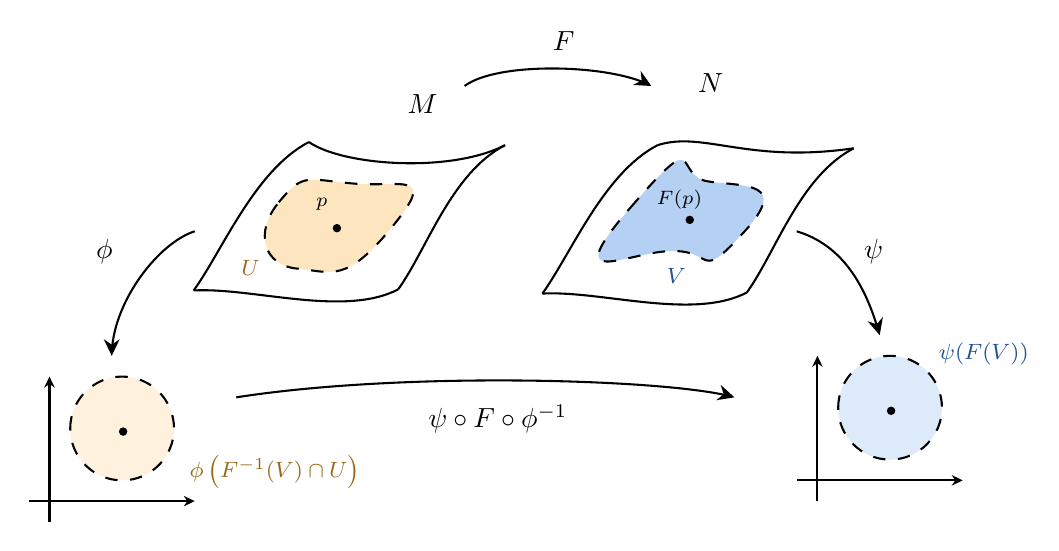
\begin{tikzpicture}[x=0.75pt,y=0.75pt,yscale=-1,xscale=1]
		%uncomment if require: \path (0,300); %set diagram left start at 0, and has height of 300
		
		%Curve Lines [id:da11806081372332144] 
		\draw    (179.5,178.5) .. controls (193.5,159) and (209,120.5) .. (235,107) ;
		%Curve Lines [id:da18965221151827483] 
		\draw    (179.5,178.5) .. controls (208,177) and (252,191.5) .. (278,178) ;
		%Curve Lines [id:da4778597706036809] 
		\draw    (278,178) .. controls (292,158.5) and (303.5,122) .. (329.5,108.5) ;
		%Curve Lines [id:da40033578881982557] 
		\draw    (235,107) .. controls (251.5,118.5) and (303.5,122) .. (329.5,108.5) ;
		%Curve Lines [id:da8289769291382043] 
		\draw    (347.5,180) .. controls (361.5,160.5) and (377,122) .. (403,108.5) ;
		%Curve Lines [id:da562782587348567] 
		\draw    (347.5,180) .. controls (376,178.5) and (420,193) .. (446,179.5) ;
		%Curve Lines [id:da8325596531064072] 
		\draw    (446,179.5) .. controls (460,160) and (471.5,123.5) .. (497.5,110) ;
		%Curve Lines [id:da2852542457229288] 
		\draw    (403,108.5) .. controls (425,101.5) and (446.5,117.5) .. (497.5,110) ;
		%Shape: Polygon Curved [id:ds40810252904164956] 
		\draw  [fill={rgb, 255:red, 245; green, 166; blue, 35 }  ,fill opacity=0.29 ][dash pattern={on 4.5pt off 4.5pt}] (220.5,136) .. controls (232.5,121.5) and (233.5,125) .. (256.5,127) .. controls (279.5,129) and (297.5,120.5) .. (275,148) .. controls (252.5,175.5) and (246,169.5) .. (229.5,168) .. controls (213,166.5) and (208.5,150.5) .. (220.5,136) -- cycle ;
		%Shape: Polygon Curved [id:ds4832622018481927] 
		\draw  [fill={rgb, 255:red, 74; green, 144; blue, 226 }  ,fill opacity=0.41 ][dash pattern={on 4.5pt off 4.5pt}] (390,138.5) .. controls (425.5,97.5) and (410,123.5) .. (427.5,126) .. controls (445,128.5) and (467,126) .. (444.5,150.5) .. controls (422,175) and (431,159) .. (409.5,159.5) .. controls (388,160) and (354.5,179.5) .. (390,138.5) -- cycle ;
		%Straight Lines [id:da8425805433734557] 
		\draw    (110,223) -- (110,290) ;
		\draw [shift={(110,220)}, rotate = 90] [fill={rgb, 255:red, 0; green, 0; blue, 0 }  ][line width=0.08]  [draw opacity=0] (5.36,-2.57) -- (0,0) -- (5.36,2.57) -- (3.56,0) -- cycle    ;
		%Straight Lines [id:da3867027047624212] 
		\draw    (177,280) -- (100,280) ;
		\draw [shift={(180,280)}, rotate = 180] [fill={rgb, 255:red, 0; green, 0; blue, 0 }  ][line width=0.08]  [draw opacity=0] (5.36,-2.57) -- (0,0) -- (5.36,2.57) -- (3.56,0) -- cycle    ;
		%Shape: Circle [id:dp9021706695013989] 
		\draw  [fill={rgb, 255:red, 245; green, 166; blue, 35 }  ,fill opacity=0.15 ][dash pattern={on 4.5pt off 4.5pt}] (120,245) .. controls (120,231.19) and (131.19,220) .. (145,220) .. controls (158.81,220) and (170,231.19) .. (170,245) .. controls (170,258.81) and (158.81,270) .. (145,270) .. controls (131.19,270) and (120,258.81) .. (120,245) -- cycle ;
		%Straight Lines [id:da20897051537256983] 
		\draw    (480,213) -- (480,280) ;
		\draw [shift={(480,210)}, rotate = 90] [fill={rgb, 255:red, 0; green, 0; blue, 0 }  ][line width=0.08]  [draw opacity=0] (5.36,-2.57) -- (0,0) -- (5.36,2.57) -- (3.56,0) -- cycle    ;
		%Straight Lines [id:da4413765041127402] 
		\draw    (547,270) -- (470,270) ;
		\draw [shift={(550,270)}, rotate = 180] [fill={rgb, 255:red, 0; green, 0; blue, 0 }  ][line width=0.08]  [draw opacity=0] (5.36,-2.57) -- (0,0) -- (5.36,2.57) -- (3.56,0) -- cycle    ;
		%Shape: Circle [id:dp2483574720488635] 
		\draw  [fill={rgb, 255:red, 74; green, 144; blue, 226 }  ,fill opacity=0.19 ][dash pattern={on 4.5pt off 4.5pt}] (490,235) .. controls (490,221.19) and (501.19,210) .. (515,210) .. controls (528.81,210) and (540,221.19) .. (540,235) .. controls (540,248.81) and (528.81,260) .. (515,260) .. controls (501.19,260) and (490,248.81) .. (490,235) -- cycle ;
		%Curve Lines [id:da8553312339361681] 
		\draw    (310,80) .. controls (325.36,68.48) and (376.66,69.4) .. (397.55,78.78) ;
		\draw [shift={(400,80)}, rotate = 208.93] [fill={rgb, 255:red, 0; green, 0; blue, 0 }  ][line width=0.08]  [draw opacity=0] (8.04,-3.86) -- (0,0) -- (8.04,3.86) -- (5.34,0) -- cycle    ;
		%Curve Lines [id:da778090429217146] 
		\draw    (470,150) .. controls (490.75,156.27) and (502.18,173.72) .. (509.25,197.4) ;
		\draw [shift={(510,200)}, rotate = 254.36] [fill={rgb, 255:red, 0; green, 0; blue, 0 }  ][line width=0.08]  [draw opacity=0] (8.04,-3.86) -- (0,0) -- (8.04,3.86) -- (5.34,0) -- cycle    ;
		%Curve Lines [id:da210913418624189] 
		\draw    (180,150) .. controls (163.11,155.31) and (141.57,182.5) .. (140.08,207.31) ;
		\draw [shift={(140,210)}, rotate = 270] [fill={rgb, 255:red, 0; green, 0; blue, 0 }  ][line width=0.08]  [draw opacity=0] (8.04,-3.86) -- (0,0) -- (8.04,3.86) -- (5.34,0) -- cycle    ;
		%Curve Lines [id:da8925336292700183] 
		\draw    (200,230) .. controls (281,217.39) and (403.86,221.25) .. (437.17,229.25) ;
		\draw [shift={(440,230)}, rotate = 196.61] [fill={rgb, 255:red, 0; green, 0; blue, 0 }  ][line width=0.08]  [draw opacity=0] (8.04,-3.86) -- (0,0) -- (8.04,3.86) -- (5.34,0) -- cycle    ;
		%Shape: Circle [id:dp7473837647062398] 
		\draw  [fill={rgb, 255:red, 0; green, 0; blue, 0 }  ,fill opacity=1 ] (247,148.5) .. controls (247,147.67) and (247.67,147) .. (248.5,147) .. controls (249.33,147) and (250,147.67) .. (250,148.5) .. controls (250,149.33) and (249.33,150) .. (248.5,150) .. controls (247.67,150) and (247,149.33) .. (247,148.5) -- cycle ;
		%Shape: Circle [id:dp9244279482747275] 
		\draw  [fill={rgb, 255:red, 0; green, 0; blue, 0 }  ,fill opacity=1 ] (417,144.5) .. controls (417,143.67) and (417.67,143) .. (418.5,143) .. controls (419.33,143) and (420,143.67) .. (420,144.5) .. controls (420,145.33) and (419.33,146) .. (418.5,146) .. controls (417.67,146) and (417,145.33) .. (417,144.5) -- cycle ;
		%Shape: Circle [id:dp5699925804076371] 
		\draw  [fill={rgb, 255:red, 0; green, 0; blue, 0 }  ,fill opacity=1 ] (144,246.5) .. controls (144,245.67) and (144.67,245) .. (145.5,245) .. controls (146.33,245) and (147,245.67) .. (147,246.5) .. controls (147,247.33) and (146.33,248) .. (145.5,248) .. controls (144.67,248) and (144,247.33) .. (144,246.5) -- cycle ;
		%Shape: Circle [id:dp11209906657188418] 
		\draw  [fill={rgb, 255:red, 0; green, 0; blue, 0 }  ,fill opacity=1 ] (514,236.5) .. controls (514,235.67) and (514.67,235) .. (515.5,235) .. controls (516.33,235) and (517,235.67) .. (517,236.5) .. controls (517,237.33) and (516.33,238) .. (515.5,238) .. controls (514.67,238) and (514,237.33) .. (514,236.5) -- cycle ;
		
		% Text Node
		\draw (281,82.4) node [anchor=north west][inner sep=0.75pt]    {$M$};
		% Text Node
		\draw (421,72.4) node [anchor=north west][inner sep=0.75pt]    {$N$};
		% Text Node
		\draw (351,52.4) node [anchor=north west][inner sep=0.75pt]    {$F$};
		% Text Node
		\draw (501,152.4) node [anchor=north west][inner sep=0.75pt]    {$\psi $};
		% Text Node
		\draw (131,152.4) node [anchor=north west][inner sep=0.75pt]    {$\phi $};
		% Text Node
		\draw (291,232.4) node [anchor=north west][inner sep=0.75pt]    {$\psi \circ F\circ \phi ^{-1}$};
		% Text Node
		\draw (237,132.4) node [anchor=north west][inner sep=0.75pt]  [font=\scriptsize]  {$p$};
		% Text Node
		\draw (401,128.4) node [anchor=north west][inner sep=0.75pt]  [font=\scriptsize]  {$F( p)$};
		% Text Node
		\draw (201,162.4) node [anchor=north west][inner sep=0.75pt]  [font=\footnotesize,color={rgb, 255:red, 155; green, 104; blue, 25 }  ,opacity=1 ]  {$U$};
		% Text Node
		\draw (406,166.4) node [anchor=north west][inner sep=0.75pt]  [font=\footnotesize,color={rgb, 255:red, 29; green, 81; blue, 148 }  ,opacity=1 ]  {$V$};
		% Text Node
		\draw (537,202.4) node [anchor=north west][inner sep=0.75pt]  [font=\footnotesize,color={rgb, 255:red, 29; green, 81; blue, 148 }  ,opacity=1 ]  {$\psi ( F( V))$};
		% Text Node
		\draw (176,256.4) node [anchor=north west][inner sep=0.75pt]  [font=\footnotesize,color={rgb, 255:red, 155; green, 104; blue, 25 }  ,opacity=1 ]  {$\phi \left( F^{-1}( V) \cap U\right)$};
		
		
	\end{tikzpicture}
\end{figure}